\documentclass{standalone}
\usepackage{tikz}
\usetikzlibrary{patterns, positioning}


\begin{document}
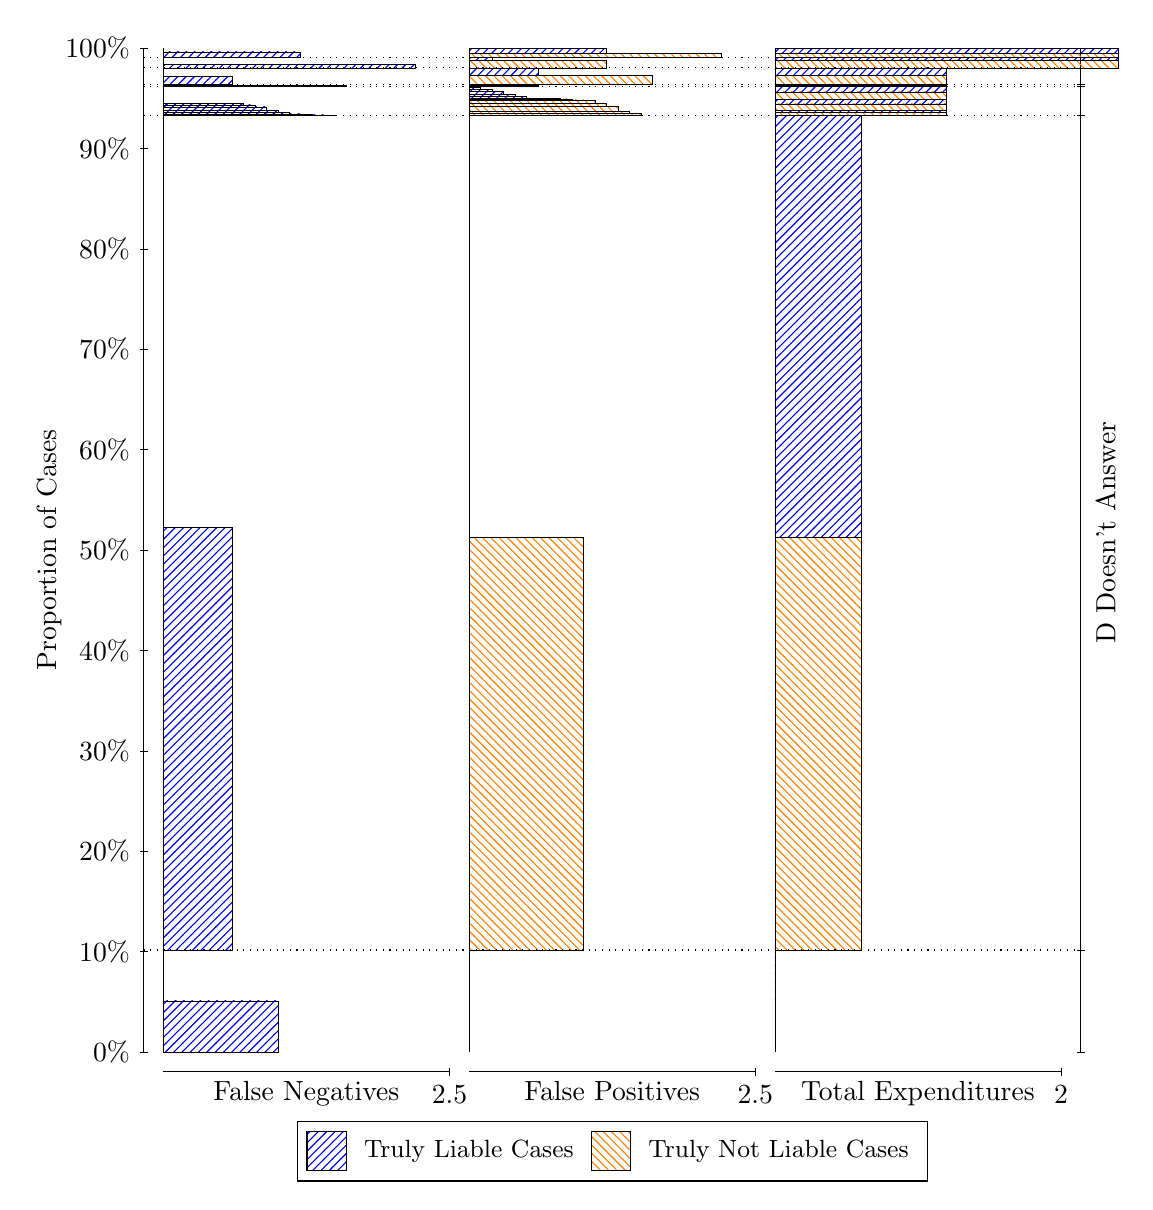
\begin{tikzpicture}
\draw[black, very thin] (1.5,1.75) -- (1.5,14.5);
\node[rotate=90, text=black, anchor=center] at (0.3, 8.125) {Proportion of Cases};
\draw[black, very thin] (1.45,1.75) -- (1.55,1.75);
\node[text=black, anchor=east] at (1.45, 1.75) {0\%};
\draw[black, very thin] (1.45,3.025) -- (1.55,3.025);
\node[text=black, anchor=east] at (1.45, 3.025) {10\%};
\draw[black, very thin] (1.45,4.3) -- (1.55,4.3);
\node[text=black, anchor=east] at (1.45, 4.3) {20\%};
\draw[black, very thin] (1.45,5.575) -- (1.55,5.575);
\node[text=black, anchor=east] at (1.45, 5.575) {30\%};
\draw[black, very thin] (1.45,6.85) -- (1.55,6.85);
\node[text=black, anchor=east] at (1.45, 6.85) {40\%};
\draw[black, very thin] (1.45,8.125) -- (1.55,8.125);
\node[text=black, anchor=east] at (1.45, 8.125) {50\%};
\draw[black, very thin] (1.45,9.4) -- (1.55,9.4);
\node[text=black, anchor=east] at (1.45, 9.4) {60\%};
\draw[black, very thin] (1.45,10.675) -- (1.55,10.675);
\node[text=black, anchor=east] at (1.45, 10.675) {70\%};
\draw[black, very thin] (1.45,11.95) -- (1.55,11.95);
\node[text=black, anchor=east] at (1.45, 11.95) {80\%};
\draw[black, very thin] (1.45,13.225) -- (1.55,13.225);
\node[text=black, anchor=east] at (1.45, 13.225) {90\%};
\draw[black, very thin] (1.45,14.5) -- (1.55,14.5);
\node[text=black, anchor=east] at (1.45, 14.5) {100\%};

\draw[black, very thin] (13.4,1.75) -- (13.4,14.5);
\draw[black, very thin] (13.35,1.75) -- (13.45,1.75);
\node[anchor=west] at (13.35, 1.75) {};
\draw[black, very thin] (13.35,3.0455) -- (13.45,3.0455);
\node[anchor=west] at (13.35, 3.0455) {};
\draw[black, very thin] (13.35,13.645) -- (13.45,13.645);
\node[anchor=west] at (13.35, 13.645) {};
\draw[black, very thin] (13.35,14.016) -- (13.45,14.016);
\node[anchor=west] at (13.35, 14.016) {};
\draw[black, very thin] (13.35,14.041) -- (13.45,14.041);
\node[anchor=west] at (13.35, 14.041) {};
\draw[black, very thin] (13.35,14.249) -- (13.45,14.249);
\node[anchor=west] at (13.35, 14.249) {};
\draw[black, very thin] (13.35,14.383) -- (13.45,14.383);
\node[anchor=west] at (13.35, 14.383) {};
\draw[black, very thin] (13.35,14.5) -- (13.45,14.5);
\node[anchor=west] at (13.35, 14.5) {};

\draw[black, very thin, pattern color=blue, pattern=north east lines] (1.75,1.75) rectangle (3.2033,2.3978);
\draw[black, very thin, pattern color=orange, pattern=north west lines] (1.75,2.3978) rectangle (1.75,3.0455);
\draw[black, very thin, pattern color=blue, pattern=north east lines] (1.75,3.0455) rectangle (2.622,8.4075);
\draw[black, very thin, pattern color=orange, pattern=north west lines] (1.75,8.4075) rectangle (1.75,13.645);
\draw[black, very thin, pattern color=blue, pattern=north east lines] (1.75,13.645) rectangle (3.93,13.648);
\draw[black, very thin, pattern color=blue, pattern=north east lines] (1.75,13.648) rectangle (3.7847,13.652);
\draw[black, very thin, pattern color=blue, pattern=north east lines] (1.75,13.652) rectangle (3.6393,13.658);
\draw[black, very thin, pattern color=blue, pattern=north east lines] (1.75,13.658) rectangle (3.494,13.664);
\draw[black, very thin, pattern color=blue, pattern=north east lines] (1.75,13.664) rectangle (3.3487,13.687);
\draw[black, very thin, pattern color=blue, pattern=north east lines] (1.75,13.687) rectangle (3.2033,13.707);
\draw[black, very thin, pattern color=blue, pattern=north east lines] (1.75,13.707) rectangle (3.058,13.752);
\draw[black, very thin, pattern color=blue, pattern=north east lines] (1.75,13.752) rectangle (2.9127,13.779);
\draw[black, very thin, pattern color=blue, pattern=north east lines] (1.75,13.779) rectangle (2.7673,13.798);
\draw[black, very thin, pattern color=orange, pattern=north west lines] (1.75,13.798) rectangle (1.75,14.016);
\draw[black, very thin, pattern color=blue, pattern=north east lines] (1.75,14.016) rectangle (4.0753,14.025);
\draw[black, very thin, pattern color=orange, pattern=north west lines] (1.75,14.025) rectangle (1.75,14.041);
\draw[black, very thin, pattern color=blue, pattern=north east lines] (1.75,14.041) rectangle (2.622,14.135);
\draw[black, very thin, pattern color=orange, pattern=north west lines] (1.75,14.135) rectangle (1.75,14.249);
\draw[black, very thin, pattern color=blue, pattern=north east lines] (1.75,14.249) rectangle (4.9473,14.291);
\draw[black, very thin, pattern color=orange, pattern=north west lines] (1.75,14.291) rectangle (1.75,14.383);
\draw[black, very thin, pattern color=blue, pattern=north east lines] (1.75,14.383) rectangle (3.494,14.451);
\draw[black, very thin, pattern color=orange, pattern=north west lines] (1.75,14.451) rectangle (1.75,14.5);
\draw[black, very thin, pattern color=orange, pattern=north west lines] (5.6333,1.75) rectangle (5.6333,2.3978);
\draw[black, very thin, pattern color=blue, pattern=north east lines] (5.6333,2.3978) rectangle (5.6333,3.0455);
\draw[black, very thin, pattern color=orange, pattern=north west lines] (5.6333,3.0455) rectangle (7.0867,8.2834);
\draw[black, very thin, pattern color=blue, pattern=north east lines] (5.6333,8.2834) rectangle (5.6333,13.645);
\draw[black, very thin, pattern color=orange, pattern=north west lines] (5.6333,13.645) rectangle (7.8133,13.666);
\draw[black, very thin, pattern color=orange, pattern=north west lines] (5.6333,13.666) rectangle (7.668,13.7);
\draw[black, very thin, pattern color=orange, pattern=north west lines] (5.6333,13.7) rectangle (7.5227,13.762);
\draw[black, very thin, pattern color=orange, pattern=north west lines] (5.6333,13.762) rectangle (7.3773,13.796);
\draw[black, very thin, pattern color=orange, pattern=north west lines] (5.6333,13.796) rectangle (7.232,13.833);
\draw[black, very thin, pattern color=orange, pattern=north west lines] (5.6333,13.833) rectangle (7.0867,13.842);
\draw[black, very thin, pattern color=orange, pattern=north west lines] (5.6333,13.842) rectangle (6.9413,13.853);
\draw[black, very thin, pattern color=orange, pattern=north west lines] (5.6333,13.853) rectangle (6.796,13.859);
\draw[black, very thin, pattern color=orange, pattern=north west lines] (5.6333,13.859) rectangle (6.6507,13.863);
\draw[black, very thin, pattern color=blue, pattern=north east lines] (5.6333,13.863) rectangle (6.36,13.882);
\draw[black, very thin, pattern color=blue, pattern=north east lines] (5.6333,13.882) rectangle (6.2147,13.909);
\draw[black, very thin, pattern color=blue, pattern=north east lines] (5.6333,13.909) rectangle (6.0693,13.954);
\draw[black, very thin, pattern color=blue, pattern=north east lines] (5.6333,13.954) rectangle (5.924,13.974);
\draw[black, very thin, pattern color=blue, pattern=north east lines] (5.6333,13.974) rectangle (5.7787,13.997);
\draw[black, very thin, pattern color=blue, pattern=north east lines] (5.6333,13.997) rectangle (5.6333,14.016);
\draw[black, very thin, pattern color=orange, pattern=north west lines] (5.6333,14.016) rectangle (6.5053,14.032);
\draw[black, very thin, pattern color=blue, pattern=north east lines] (5.6333,14.032) rectangle (5.6333,14.041);
\draw[black, very thin, pattern color=orange, pattern=north west lines] (5.6333,14.041) rectangle (7.9587,14.155);
\draw[black, very thin, pattern color=blue, pattern=north east lines] (5.6333,14.155) rectangle (6.5053,14.249);
\draw[black, very thin, pattern color=orange, pattern=north west lines] (5.6333,14.249) rectangle (7.3773,14.341);
\draw[black, very thin, pattern color=blue, pattern=north east lines] (5.6333,14.341) rectangle (5.924,14.383);
\draw[black, very thin, pattern color=orange, pattern=north west lines] (5.6333,14.383) rectangle (8.8307,14.432);
\draw[black, very thin, pattern color=blue, pattern=north east lines] (5.6333,14.432) rectangle (7.3773,14.5);
\draw[black, very thin, pattern color=orange, pattern=north west lines] (9.5167,1.75) rectangle (9.5167,2.3978);
\draw[black, very thin, pattern color=blue, pattern=north east lines] (9.5167,2.3978) rectangle (9.5167,3.0455);
\draw[black, very thin, pattern color=orange, pattern=north west lines] (9.5167,3.0455) rectangle (10.607,8.2834);
\draw[black, very thin, pattern color=blue, pattern=north east lines] (9.5167,8.2834) rectangle (10.607,13.645);
\draw[black, very thin, pattern color=orange, pattern=north west lines] (9.5167,13.645) rectangle (11.697,13.683);
\draw[black, very thin, pattern color=blue, pattern=north east lines] (9.5167,13.683) rectangle (11.697,13.706);
\draw[black, very thin, pattern color=orange, pattern=north west lines] (9.5167,13.706) rectangle (11.697,13.79);
\draw[black, very thin, pattern color=blue, pattern=north east lines] (9.5167,13.79) rectangle (11.697,13.848);
\draw[black, very thin, pattern color=orange, pattern=north west lines] (9.5167,13.848) rectangle (11.697,13.944);
\draw[black, very thin, pattern color=blue, pattern=north east lines] (9.5167,13.944) rectangle (11.697,14.016);
\draw[black, very thin, pattern color=orange, pattern=north west lines] (9.5167,14.016) rectangle (11.697,14.032);
\draw[black, very thin, pattern color=blue, pattern=north east lines] (9.5167,14.032) rectangle (11.697,14.041);
\draw[black, very thin, pattern color=orange, pattern=north west lines] (9.5167,14.041) rectangle (11.697,14.155);
\draw[black, very thin, pattern color=blue, pattern=north east lines] (9.5167,14.155) rectangle (11.697,14.249);
\draw[black, very thin, pattern color=orange, pattern=north west lines] (9.5167,14.249) rectangle (13.877,14.341);
\draw[black, very thin, pattern color=blue, pattern=north east lines] (9.5167,14.341) rectangle (13.877,14.383);
\draw[black, very thin, pattern color=orange, pattern=north west lines] (9.5167,14.383) rectangle (13.877,14.432);
\draw[black, very thin, pattern color=blue, pattern=north east lines] (9.5167,14.432) rectangle (13.877,14.5);
\draw[black, dotted] (1.5,3.0455) -- (13.4,3.0455);
\draw[black, dotted] (1.5,13.645) -- (13.4,13.645);
\draw[black, dotted] (1.5,14.016) -- (13.4,14.016);
\draw[black, dotted] (1.5,14.041) -- (13.4,14.041);
\draw[black, dotted] (1.5,14.249) -- (13.4,14.249);
\draw[black, dotted] (1.5,14.383) -- (13.4,14.383);
\draw[black, very thin] (1.75,1.5) -- (5.3833,1.5);
\node[text=black, anchor=north] at (3.5667, 1.5) {False Negatives};
\draw[black, very thin] (5.3833,1.45) -- (5.3833,1.55);
\node[text=black, anchor=north] at (5.3833, 1.45) {2.5};

\draw[black, very thin] (5.6333,1.5) -- (9.2667,1.5);
\node[text=black, anchor=north] at (7.45, 1.5) {False Positives};
\draw[black, very thin] (9.2667,1.45) -- (9.2667,1.55);
\node[text=black, anchor=north] at (9.2667, 1.45) {2.5};

\draw[black, very thin] (9.5167,1.5) -- (13.15,1.5);
\node[text=black, anchor=north] at (11.333, 1.5) {Total Expenditures};
\draw[black, very thin] (13.15,1.45) -- (13.15,1.55);
\node[text=black, anchor=north] at (13.15, 1.45) {2};


\node[text=black, centered, rotate=90] at (13.72, 8.3454) {D Doesn't Answer};






\draw (7.449999999999999,1.5) node[draw=none] (baseCoordinate) {};
\begin{scope}[align=center]
        \matrix[scale=0.5, draw=black, below=0.5cm of baseCoordinate, nodes={draw}, column sep=0.1cm]{
            \node[rectangle, draw, minimum width=0.5cm, minimum height=0.5cm, pattern color=blue, pattern=north east lines] {}; &
            \node[draw=none, font=\small, text=black] (B) {Truly Liable Cases}; &
            \node[rectangle, draw, minimum width=0.5cm, minimum height=0.5cm, pattern color=orange, pattern=north west lines] {}; &
            \node[draw=none, font=\small, text=black] (B) {Truly Not Liable Cases}; \\
            };
\end{scope}

\end{tikzpicture}
\end{document}